\documentclass{article}
\usepackage{graphicx} % Required for inserting images
\usepackage{amsmath}
\usepackage{amssymb}
\usepackage{mathtools}
\usepackage{mathrsfs}
\usepackage{titletoc}
\usepackage{tikz}
\usepackage{fourier-orns}
\usepackage{fancyhdr}
\usepackage[margin=1cm]{geometry}
\usepackage[most]{tcolorbox}
\usepackage{hyperref}
\hypersetup{
    colorlinks=true,
    linkcolor=blue,
    filecolor=magenta,      
    urlcolor=cyan,
    pdftitle={Overleaf Example},
    pdfpagemode=FullScreen,
    }
\urlstyle{same}
\newcommand{\R}{\mathbb{R}}
\newcommand{\BAB}{\mathbb{\big\vert}}
\newcommand{\NN}{\mathbb{N}}
\newcommand{\Ss}{\\ \vspace{2mm}}
\newcommand{\NL}{\newline 
\newline}
\newcommand{\EX}{\mathbb{E}}
\newcommand{\PR}{\mathbb{P}}
\renewcommand{\headrule}{%
\vspace{-8pt}\hrulefill
\raisebox{-2.1pt}{\quad\decofourleft\decotwo\decofourright\quad}\hrulefill}
\geometry{
    left=1cm,
    top=1in,
    right=1cm,
    bottom=1cm
}

\fancyhf{}
\newcommand{\papertitle}{Neural Network Gaussian Process and Conjugate Kernels}
\fancyhead[LE]{\thepage}
\fancyhead[RE]{\papertitle}
\fancyhead[LO]{\papertitle}
\fancyhead[RO]{\thepage}

\begin{document}
\pagenumbering{gobble}
\begin{titlepage}
    \begin{center}
        \hspace{0pt}\\
        {\scalebox{2}{\Huge\bfseries NEURAL}}\\
        \vspace{4mm}
        {\scalebox{2}{\Huge\bfseries NETWORK}}\\
        \vspace{4mm}
        {\scalebox{2}{\Huge\bfseries GAUSSIAN}}\\
        \vspace{4mm}
        {\scalebox{2}{\Huge\bfseries PROCESS}}\\
        \vspace{4mm}
        {\scalebox{2}{\Huge\bfseries AND}}\\
        \vspace{4mm}
        {\scalebox{2}{\Huge\bfseries CONJUGATE}}\\
        \vspace{4mm}
        {\scalebox{2}{\Huge\bfseries KERNELS}}\\
        \vspace{0.8cm}
        {\Large\bfseries PROFESSOR ALEXANDER CLONINGER}\\[5pt]
        \vspace{4mm}
        {\Large\bfseries TRISTAN ENDO}\\[5pt]
        \vspace{3mm}
        \begin{figure}[h]
            \centering
            \includegraphics[width=0.4\linewidth]{UCSD seal.png}
        \end{figure}
         \vfill
         University of California, San Diego\\
         United States—2026
    \end{center}
\end{titlepage}
\pagestyle{empty}
\tableofcontents
\pagebreak
\pagestyle{fancy}
\pagenumbering{arabic}
\setcounter{page}{1} 
\section{Introduction and Contributions}
In recent years, modern deep neural networks have been empirically successful in machine learning tasks. Still, the theoretical understanding of neural network generalization and how architectures impact function learning remains limited. One approach to analyzing these neural networks is taking the \textit{infinite-width limit}, where randomly initialized neural networks converge to Gaussian processes. Under this approach, predictions can be described via a kernel function, determined by network architecture and activation function.
\NL
The connection between neural networks and Gaussian processes dates back to 1996, when \textit{Radford M. Neal} proposed that single-layer neural networks with randomized weights converge to a Gaussian process when the limit of the widths is taken to $\infty$. A detailed explanation can be found in his work, \href{https://glizen.com/radfordneal/bnn.book.html}{\textit{Bayesian Learning for Neural Networks}}. After some time, in 2018, \textit{Jaehoon Lee} and collaborators extended this discovery to deep neural networks in their paper, \href{https://arxiv.org/abs/1711.00165}{\textit{Deep Neural Networks as Gaussian Processes}}. In particular, outputs of a randomly initialized deep neural network converge to a \textit{Neural Network Gaussian Process}, or the \textit{NNGP}, whose covariance kernel evolves recursively across network layers.
\NL
The \textit{NNGP} provides a rigorous tool for analyzing neural network function spaces and reveals a tight relationship between neural networks and kernel methods. More specifically, the covariance kernels produced by infinite-width networks depend on the activation function chosen in addition to the parameters of the architecture: depth, weight variance, and normalized inputs. These kernels, also referred to as \textit{conjugate kernels} in literature, can determine the class of functions that the infinite-width network can effectively represent and therefore characterize the learning bias.
\NL
In this project, we investigate the architecture and behavior of NNGP against the activation functions: \textit{Rectified Linear Unit (ReLU), Gauss Error Function (erf)}, and the \textit{Hyperbolic Tangent (tanh)}. We will derive the corresponding closed-form conjugate kernels and examine how they evolve recursively layer by layer. Furthermore, we analyze how the depth, weight variance, and normalized inputs affect kernel degeneracy, spectral bias, and expressivity. Finally, we will compare NNGP predictions with finite-width neural networks to see when the kernel methods accurately approximate behavior and when deviations indicate feature learning beyond the conjugate kernel regime.

\section{Definitions}
\subsection{Neural Networks and Infinite-Width Limits}
Consider a fully connected \textit{feedforward neural network} of depth $L$. Given an input $x\in \R^d$, the activations in a layer $l$ is defined recursively by 
$$g^{(l)}(y)=\phi(W^{(l)}g^{(l-1)}(y)+b^{(l)})$$
Here, $W^{(l)}$ and $b^{(l)}$ represent the weight matrix and bias vector, respectively, for layer $l$ and $\phi(\cdot)$ is the chosen nonlinear activation function. To ensure stability per layer, weights are initialized according to a Gaussian distribution with mean 0 and variance $(\sigma^2_w/\text{width of the previous layer})$. That is,
$$W^{(l)}_{ij}\sim \mathcal{N}\Bigg(0,\frac{\sigma_w^2}{n_{l-1}}\Bigg)\qquad n_{l-1}=\text{width of the preceding layer}$$
Taking the limit of the width $n_l\to \infty$, each $W^{(l)}g^{(l-1)}(y)+b^{(l)}$ becomes a sum of many independent random variables. Under the \textit{Central Limit Theorem}, each $W^{(l)}g^{(l-1)}(y)+b^{(l)}$ converges in distribution to a Gaussian random variable. As such, the neural network outputs converge to a \textit{Gaussian Process} whose covariance function is dependent on the inputs and the network architecture.
\subsection{Neural Network Gaussian Process (NNGP)}
In the infinite-width limit, the covariance between the outputs corresponding to two units, $y,y'$ is given via a kernel, defined as the following,
$$K^{(l)}(y,y')=Cov\Big(g^{(l)}(y),g^{(l)}(y')\Big)$$
where on a fully connected neural network, it evolves recursively across layers according to
$$K^{(l+1)}(y,y')=\sigma^2_b+\sigma^2_w\cdot\EX_{(u,v)\sim \mathcal{N}(0,\Sigma)}[\phi(u)\phi(v)]\qquad \text{with}\qquad \Sigma=\begin{bmatrix}
    K^{(l)}(y,y) & K^{(l)}(y,y')\\
    K^{(l)}(y',y) & K^{(l)}(y',y')
\end{bmatrix}$$
This is the \textit{Neural Network Gaussian Process Kernel}, which determines the distribution of functions on infinite-width networks. The choice of activation functions will produce different closed-form kernels, which is derived from taking the Gaussian expectation in the recursion.
\NL
The kernel describes how neural networks transform input correlations using depth to reveal properties such as expressivity and learning bias.

\section{Closed-Form Conjugate Kernels}
We will define the Neural Network Gaussian Process kernel recursively by taking the Gaussian expectation of the activation outputs when $(u,v)$, are jointly Gaussian, $\EX[\phi(u)\phi(v)]$. The pair $(u,v)$ has a covariance matrix determined by the kernel of the previous layer. The expectation evaluates how the input correlation changes layer by layer.
\NL
For commonly used activation functions, the expectations can be computed analytically, producing a closed-form expression of the kernel. These expressions are referred to as the \textit{conjugate kernels}. The exact form of the conjugate kernels depends on the activation function used in the neural network, and it determines the set of functions the infinite-width network can represent. In other words, the kernel determines what kind of input-output relationships the network can learn.
\NL
To investigate the kernels, it is convenient to express the recursion in terms of the correlation between two inputs. This normalization removes the dependence on the magnitudes of the inputs and reduces the problem to a one-dimensional system, which describes how similarities between inputs evolve layer by layer. Define the kernel at layer $l$ by $K^{(l)}(y,y')$ where $y$ and $y'$ are two inputs, the corresponding correlation, $\rho$, 
$$\rho^{(l)}(y,y')=\frac{K^{(l)}(y,y')}{\sqrt{K^{(l)}(y,y)\cdot K^{(l)}(y',y')}}$$
The \textit{correlation coefficient} describes how similar the representations of two inputs are at each layer of the neural network.
\subsection{Rectified Linear Unit (ReLU) Conjugate Kernel}
Consider the \textit{Rectified Linear Unit (ReLU)} activation function, denoted by $\phi(z)=\max(0,z)$. When inputs, $y,y'$ are jointly Gaussian with correlation $\rho$, the expectation can be analytically evaluated. Because ReLU is zero for non-positive constants, the integral is reduced to the positive quadrant.
\begin{align}
    \EX[\phi(u)\phi(v)]=\int_{\R^2}\phi(u)\phi(v)\rho(u,v)~du~dv=\int_0^\infty\int_0^\infty uv\rho(u,v)~du~dv
\end{align}
The exact integral was computed by \href{https://papers.nips.cc/paper/2009/hash/5751ec3e9a4feab575962e78e006250d-Abstract.html}{\textit{Youngmin Cho \& Lawrence Saul (2009)}}. They called the expectation the \textit{arc-cosine kernel} which after evaluating the integrals, we get that if we let $c$ be the correlation between $u$ and $v$,
$$\EX[\phi(u)\phi(v)]=\frac{\sqrt{1-c^2}+c(\pi-\arccos(c))}{2\pi}$$
Substituting this expression back into the recursive formula produces the \textit{ReLU kernel}, which can be written in terms of the angle between the two input vectors. The resulting \textit{ReLU conjugate kernel} is computed in \textit{Jaehoon Lee (2018)} 
$$K^{(l+1)}(y,y')=\sigma_b^2+\frac{\sigma_w^2}{2\pi}\sqrt{K^{(l)}(y,y)K^{(l)}(y',y')}\Bigg(\sin\theta^{l}_{y,y'}+(\pi-\theta_{y,y'}^{l})\cos\theta^{l}_{y,y'}\Bigg)$$
$$\theta^l_{y,y'}=\arccos\Bigg(\frac{K^{(l)}(y,y')}{\sqrt{(K^{(l)}(y,y))\cdot (K^{(l)}(y',y'))}}\Bigg)$$
The \textit{ReLU conjugate kernel} is similar to that of the arc-cosine kernel and depends on the geometric relationship between the two inputs $y,y'$. Since ReLU is a piecewise linear function, the resulting kernel induces functions that are composed of piecewise linear transformations of the inputs.
\subsection{Gauss Error Function (erf) Conjugate Kernel}
Another common activation function is the \textit{Gauss Error Function (erf)}, denoted by $\phi(z)=erf(z)$ where
$$erf(z)=\frac{2}{\sqrt{\pi}}\int_0^ze^{-t^2}~dt$$
The closed-form kernel from sigmoidal activation functions was first derived by \textit{Christopher Williams (1996)} in his work \href{https://papers.nips.cc/paper/1996/hash/ae5e3ce40e0404a45ecacaaf05e5f735-Abstract.html}{\textit{Computing with Infinite Networks}}. Following the formulation, the expectation of the kernel can be expressed as an integral over the distribution of the network weights. Let $u\sim \mathcal{N}(0,\Sigma)$ be a random weight vector, where $\Sigma$ is the covariance matrix, and let $\tilde{x}=(1,x_1,\cdots,x_d)$ be an augmented input vector whose first entry corresponds to the bias. Then,
$$\EX[\phi(x;u)\phi(x';u)]=\frac{1}{\sqrt{(2\pi)^{d+1}|\Sigma|}}\cdot \int\phi(u^T\tilde{x})\phi(u^T\tilde{x}')\cdot \exp\Bigg(-\frac{u^T\Sigma^{-1}u}{2}\Bigg)~du$$
Evaluating the integral analytically yields
$$\EX[\phi(x;u)\phi(x';u)]=\frac{2}{\pi}\arcsin\Bigg(\frac{2\tilde{x}^T\Sigma \tilde{x}'}{\sqrt{(1+2\tilde{x}^T\Sigma \tilde{x})(1+2\tilde{x}'^T\Sigma \tilde{x}')}}\Bigg)$$
Finally, substituting it back into the recursive formula, the closed-form expression for the \textit{erf conjugate kernel} with two input vectors $y,y'$ produces what is known as the \textit{arc-sine kernel}, which shows up when Gaussian weights are combined with sigmoidal activation functions.
$$K^{(l+1)}(y,y')=\sigma_b^2+\frac{2\sigma_w^2}{\pi}\arcsin\Bigg(\frac{K^{(l)}(y,y')}{\sqrt{(K^{(l)}(y,y))\cdot (K^{(l)}(y',y'))}}\Bigg)$$
$$K^{(l)}(y,y')=2\tilde{y}^T\Sigma^{(l-1)} \tilde{y}'\qquad K^{(l)}(y,y)=1+2\tilde{y}^T\Sigma^{(l-1)} \tilde{y}\qquad K^{(l)}(y',y')=1+2\tilde{y}'^T\Sigma^{(l-1)} \tilde{y}'$$
\subsection{Hyperbolic Tangent (tanh) Conjugate Kernel}
The last activation function we will investigate is the \textit{hyperbolic tangent (tanh)}, denoted by $\phi(z)=\tanh(z)$ 
$$\tanh(z)=\frac{e^{2z}-1}{e^{2z}+1}$$
The expectation becomes $\EX_{(u,v)\sim \mathcal{N}(0,\Sigma)}[\tanh(u)\tanh(v)]$ with $u,v\sim \mathcal{N}(0,\Sigma)$. Plugging back into the recursive formula, we get that the \textit{Hyperbolic Tangent conjugate kernel} is 
$$K^{(l+1)}(y,y')=\sigma_b^2+\sigma_w^2\cdot \EX_{(u,v)\sim \mathcal{N}(0,\Sigma)}[\tanh(u)\tanh(v)]$$
Unfortunately, the hyperbolic tangent activation function cannot produce a closed-form expression for the kernel. This is because the expectation does not produce a simple analytic closed form expression under the bivariate Gaussian distribution. For example, ReLU is piecewise linear whose integrals can be solved analytically. The erf produces a Gaussian integral, which simplifies nicely, as seen above. However, tanh is a ratio of exponentials whose integrals tend to be messy. Thus, the expectation is solved numerically (or approximated by series expansion), and in literature it is left in implicit form. The \textit{hyperbolic tangent conjugate kernel} in recursive form remains
$$K^{(l+1)}(y,y')=\sigma_b^2+\sigma_w^2\cdot \EX_{(u,v)\sim \mathcal{N}(0,\Sigma)}[\tanh(u)\tanh(v)]$$
where $\Sigma$ is the covariance matrix of the previous layer.
\section{Kernel Recursion and Depth Dynamics}
\subsection{Kernel Recursion and Input Correlation}
The recursive kernel formulation provides a valuable understanding on how the representations evolve layer by layer. For two input vectors, $y,y'\in \R^d$, the kernel at layer $l$, $K^{(l)}(y,y')$ determines the covariance between their hidden layer activations. Recall that the recursion can be expressed in terms of the correlation between two inputs. Substituting the closed-form expectations of the examined activation functions produces a \textit{one-dimensional recursive map}. Using $\rho^{(l)}$ to be the correlation coefficient between two inputs, $\rho^{(l)}=F(\rho^{(l-1)})$, where $F$ depends on the activation function in addition to the weight and bias variance, $\sigma^2_w$ and $\sigma_b^2$, respectively. This construction allows us to study the transformation of similarities between inputs as they travel through successive layers. To illustrate how representations evolve through depth, consider the following diagram of a three-layer neural network.
\begin{center}
    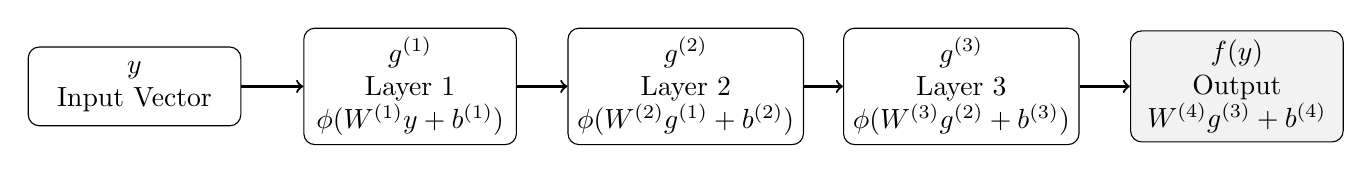
\begin{tikzpicture}[
    node distance=3.5cm,
    every node/.style={draw, rectangle, rounded corners, align=center, minimum width=2.7cm, minimum height=1cm},
    arrow/.style={->, thick}
    ]
    
    \node (input) {$y$ \\ Input Vector};
    
    \node (layer1) [right of=input] {$g^{(1)}$ \\ Layer 1 \\ $\phi(W^{(1)}y+b^{(1)})$};
    
    \node (layer2) [right of=layer1] {$g^{(2)}$ \\ Layer 2 \\ $\phi(W^{(2)}g^{(1)}+b^{(2)})$};
    
    \node (layer3) [right of=layer2] {$g^{(3)}$ \\ Layer 3 \\ $\phi(W^{(3)}g^{(2)}+b^{(3)})$};

    \node (output) [right of=layer3, fill=gray!10] {$f(y)$ \\ Output \\ $W^{(4)}g^{(3)}+b^{(4)}$};
    
    \draw[arrow] (input) -- (layer1);
    \draw[arrow] (layer1) -- (layer2);
    \draw[arrow] (layer2) -- (layer3);
    \draw[arrow] (layer3) -- (output);
    
    \end{tikzpicture}
\end{center}

\[
g^{(l)} =
\underbrace{
\phi\left(
\underbrace{W^{(l)}g^{(l-1)} + b^{(l)}}_{\begin{array}{c}
\text{network applies weights}
\end{array}}
\right)
}_{\begin{array}{c}
\text{applies activation} \\
\text{produces a new vector}
\end{array}}
\]
\subsection{Depth Dynamics, Kernel Degeneracy, Expressivity}
Iterating this recursion reveals that the correlation sequence converges around a \textit{fixed point}, $\rho^*$, where $\rho^*=F(\rho^*)$. Once it reaches $\rho^*$, traversing through subsequent layers no longer affects the similarities between the inputs. In many cases, $\rho^*=1$, meaning that as depth increases, the representations become highly correlated. The kernel also becomes nearly constant across inputs when it reaches this state. This is what is known as \textit{kernel degeneracy}. In this regime, the network's ability to distinguish inputs has completely deteriorated since the two inputs are near identical at $\rho^*$.
\NL
The recursion's behavior is dependent on the activation function parameters. In particular, the weight variance, $\sigma_w^2$, controls how the nonlinear transformation amplifies the correlation. For large $\sigma_w^2$, correlations rapidly converge to $1$, leading to kernel degeneracy. However, for small $\sigma_w^2$, the correlation approaches 0, and the network loses useful information about input similarities. In the middle of these extremes, there is a regime where correlation is stabilized, allowing the network to keep meaningful distinctions while still applying the nonlinear transformation.
\NL
Interpreting neural networks under the infinite-width limit relies on understanding the depth dynamics. The kernel recursion shows that the activation function and the initial parameters determine how information about inputs is passed through and if architectures retain their expressivity or collapse into trivial ones. Figure 1 visualizes how the kernel recursion transforms input similarities layer by layer and how empirical fixed points arise in finite networks.
\begin{figure}[h!]
    \centering
    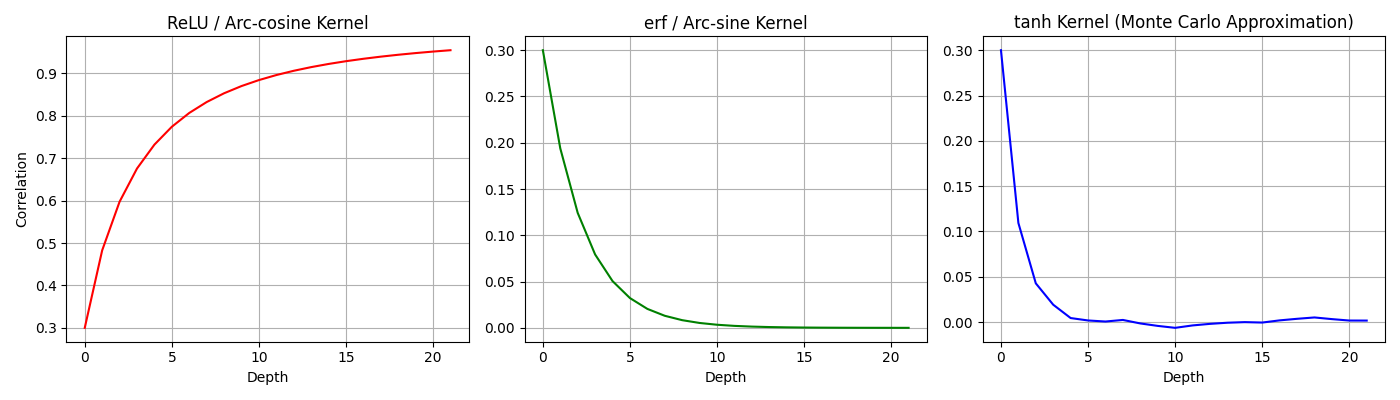
\includegraphics[width=1\linewidth]{Trig Kern.png}
    \caption{\textit{Depth dynamics of input correlations under different activation functions. It highlights the evolution of $\rho^{(l)}$ between two randomly chosen inputs as a function of network depth $l$. Here, $\rho^{(l)}$ represents the empirical fixed point for input similarities. For ReLU networks (left), the correlation rises to 1, leading to degeneracy in finite width. For erf networks (middle) and tanh networks (right), correlations decay toward zero at finite widths due to finite-width noise.}}
\end{figure}

\section{Experiments on Infinite-Width Kernels}
To investigate how depth, weight variance, and finite-width effects influence kernel behavior and neural network representations, we performed experiments on fully connected networks using the ReLU, erf, and tanh activation functions. We combined the theoretical NNGP predictions with finite-width network simulations to test when infinite-width kernels can accurately describe real networks and when deviations indicate feature learning beyond the conjugate kernel regime.
\subsection{Setup}
To start the experiment, we take a random input vector, $y,y'\in \R^{21}$, a sample from the normal distribution, normalized to unit length. This simulation focuses on fully connected networks with random initial weights sampled from a Gaussian distribution with variance scaled by the input dimensions. A depth of 10-30 layers is sufficient since it is deep enough for the correlation recursion to approach the fixed point, $\rho^*$, and the plots can clearly show degeneracy or stabilization. So, the network was fixed to a depth of 21 layers. We tested on the ReLU, erf, and tanh activation functions, and for each, networks of width 6, 36, and 216 neurons were investigated. At each layer $l$, the correlation between the hidden representations of $y,y'$ was computed by
$$\rho^{(l)}=\frac{g^{(l)}(y)\cdot g^{(l)}(y')}{||g^{(l)}(y)||\cdot ||g^{(l)}(y')||}$$
where $g^{(l)}$ is the recursive activation at layer $l$ defined in Section 2.1. This procedure was repeated through each layer to track the transformation of correlations through the network. 
\begin{figure}[h!]
    \centering
    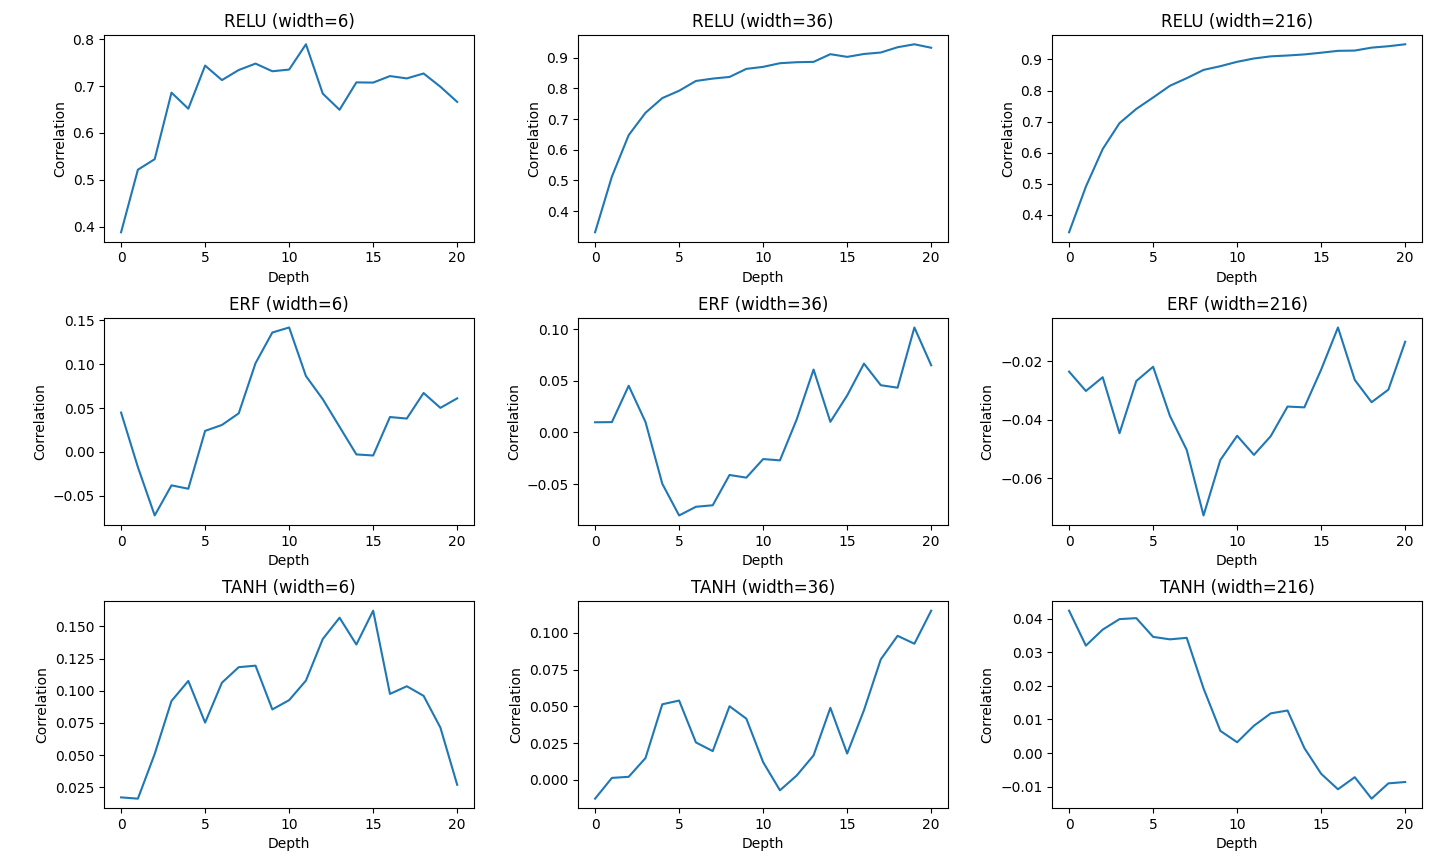
\includegraphics[width=1\linewidth]{Powers of 6 (3).png}
    \caption{\textit{Correlation dynamics for networks with widths 6, 36, 216 neurons under ReLU (left), erf (middle), and tanh (right). The correlation $\rho^{(l)}$ between two normalized inputs is tracked as a function of layer depth. As the width increases, the fluctuations from the random weights diminish, and the correlation trajectories approach the deterministic recursion predicted by the infinite-width NNGP.}}
    \label{fig:placeholder}
\end{figure}
\subsection{Effects of Activation Functions, Weight Variance, Input Normalization}
Figure 2 displays the transformation of the correlation across depth for all three activation functions with widths 6, 36, and 216. The results tell us that the activation function has a strong influence on the transformation of input similarities.
\NL
With the ReLU activation function, the correlation coefficient is monotonically increasing toward one. In other words, the representations of the different inputs have become increasingly similar. Increasing the depth, the network under the ReLU activation function produces \textit{kernel degeneracy}. On the contrary, the erf and tanh activation functions exhibit very different behavior. Correlations stabilize for smaller values of $\sigma_w^2$, meaning that the activation functions tend to decorrelate the input representations. Consequently, the network under the erf and tanh activation functions avoids kernel degeneracy and emphasizes the distinctions between two inputs. These observations illustrate how the choice of activation function influences the \textit{expressivity} of deep neural networks through kernel recursion.
\NL
This behavior toward or away from kernel degeneracy is closely related to \textit{spectral bias}. When the kernel reaches degeneracy, the kernel's eigenvalues become dominated by a small number of large eigenvalues. In kernel-based models, functions associated with larger eigenvalues tend to be learned more easily than the smaller ones. When ReLU approaches degeneracy, the kernel matrix becomes nearly constant across layers, meaning the model favors smooth functions, producing a spectral bias. However, erf and tanh tend to stabilize correlations so that more features can be represented rather than being dominated. The kernel recursion tells us a great deal about how the types of activation functions can influence the class of functions the deep network can effectively represent. 
\NL
In addition to activation choice, the kernel is also influenced by weight variances and input normalization. The weight variance parameter $\sigma_w^2$ controls how strongly correlations are emphasized across layers. Larger $\sigma_w^2$ values accelerate kernel degeneracy, while smaller values may suppress correlations. \textit{Input normalization} also influences the kernel by stabilizing it, ensuring that the correlations are dependent on angular similarity for inputs. Together, these factors determine how expressive the kernel remains as depth increases and influence the neural network's \textit{spectral bias}.
\subsection{Finite Width Effects and the Infinite-Width Limit}
The experiment reveals how network widths affect the correlation trajectory. For narrow networks (width=6), the correlation exhibits significant fluctuations due to the variations in the randomly initialized weights. As the widths get larger (36 and 216), the fluctuations lessen, and the curves become smoother.
\NL
We can conclude from this trend that for wide neural networks, as the width grows, it resembles that of the recursive kernel predicted by NNGP theory. In the infinite-width limit, the kernel transformation becomes deterministic. As a result, we can say that sufficiently wide networks can approximate the infinite-width conjugate kernel behavior.
\section{Conclusion}
While the experiments investigate randomly initialized networks, they allow us to visualize how neural networks behave under the conjugate kernel. In the infinite-width limit, training a neural network with \textit{gradient descent} can be described as kernel regression with the \textit{Neural Tangent Kernel (NTK)}, which governs the evolution of predictions during optimization. In this setting, the network learns with a fixed kernel that depends on the architecture and the activation function.
\NL
On the other hand, finite-width neural networks may deviate from this kernel regime during training. With limited width, the network parameters could alter the effective feature representation, allowing the network to learn features beyond those captured by the initial conjugate kernel. From experimentation, for neural networks to behave like the kernel, the width must be sufficiently large enough. Moreover, it emphasized how finite-width networks could deviate from this behavior through feature learning.
\section{References}
\href{https://arxiv.org/abs/1711.00165}{Jaehoon Lee, Yasaman Bahri, Roman Novak, Samuel S. Schoenholz, Jeffrey Pennington, and Jascha Sohl-Dickstein. \textit{Deep Neural Networks as Gaussian Processes}. pp. 3-6, 12-13, 2018}
\NL
\href{https://papers.nips.cc/paper/1996/hash/ae5e3ce40e0404a45ecacaaf05e5f735-Abstract.html}{Christopher K.I. Williams. Computing with Infinite Networks. \textit{In Advances in Neural Information Processing Systems}. pp. 295-301, 1997}
\NL
\href{https://papers.nips.cc/paper/2009/hash/5751ec3e9a4feab575962e78e006250d-Abstract.html}{Youngmin Cho and Lawrence K. Saul. Kernel methods for deep learning. \textit{In Advances in Neural Information Processing Systems}, pp. 342–350, 2009}
\NL
\href{https://glizen.com/radfordneal/bnn.book.html}{Radford M. Neal. \textit{Bayesian Learning for Neural Networks}. PhD thesis, University of Toronto, Dept. of Computer Science, 1994b}
\end{document}
